\documentclass{beamer}

% TikZ = desen vectorial direct in LaTeX.
\usepackage{tikz}
\usetikzlibrary{math}

% PGFPlots = grafice carteziene/polare peste TikZ.
\usepackage{pgfplots}
\usepgfplotslibrary{polar}

% Compatibilitatea recomandata pentru versiunea moderna PGFPlots.
\pgfplotsset{compat=1.18}

%Please read on the commands and options used below (either in the TikZ / PGFPlots manuals, or elsewhere).

\usepackage{filecontents}
% We're defining a file that will be created upon LaTeX compilation.
% Please note that you need to manually delete the file if you make changes,
% as filecontents does not overwrite files (for obvious security reasons).
\begin{filecontents*}{mpg.csv}
mpg,cylinders,displacement,horsepower,weight,acceleration,model_year,origin,name
18,8,307,130,3504,12,70,1,chevrolet chevelle malibu
15,8,350,165,3693,11.5,70,1,buick skylark 320
18,8,318,150,3436,11,70,1,plymouth satellite
16,8,304,150,3433,12,70,1,amc rebel sst
17,8,302,140,3449,10.5,70,1,ford torino
15,8,429,198,4341,10,70,1,ford galaxie 500
14,8,454,220,4354,9,70,1,chevrolet impala
14,8,440,215,4312,8.5,70,1,plymouth fury iii
14,8,455,225,4425,10,70,1,pontiac catalina
15,8,390,190,3850,8.5,70,1,amc ambassador dpl
15,8,383,170,3563,10,70,1,dodge challenger se
\end{filecontents*}

\begin{document}

% -----------------------------------------------------------------
% EXEMPLU 1: Primitive TikZ (linii / poligon / umplere).
% Construim doua forme simple:
%   - un triunghi albastru plin (draw + fill)
%   - un contur rosu inchis (cycle)
% -----------------------------------------------------------------
\begin{frame}
  \begin{figure}
    \center
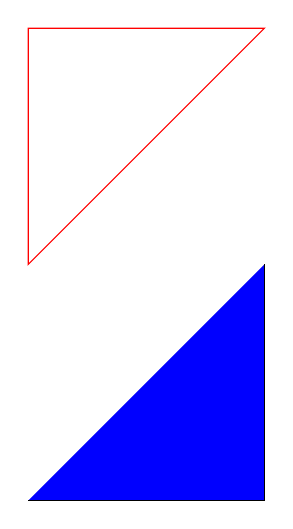
\begin{tikzpicture}[scale=3]
  \draw [fill=blue] (0, 0) -- (1, 0) -- (1, 1);
  \draw [red] (1, 2) -- (0, 2) -- (0, 1) -- cycle;
\end{tikzpicture}
    \caption{Example 1: Vector drawing in TikZ}
  \end{figure}
\end{frame}


% -----------------------------------------------------------------
% TASK 1: Hexagoane concentrice.
% CUM:
%   1) trasam un chenar patrat subtire (referinta vizuala)
%   2) desenam hexagonul mare albastru (umplut)
%   3) desenam hexagonul interior alb + contur rosu
% Observatie: coordonatele de forma (60:R), (0:R), ... sunt in sistem polar.
% -----------------------------------------------------------------
\begin{frame}
  \begin{figure}
    \center
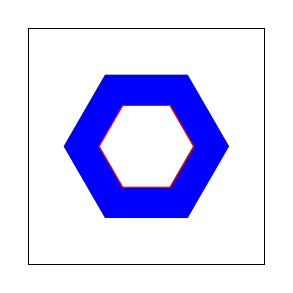
\begin{tikzpicture}[scale=3]
  \draw[black, thin] (-0.5,-0.5) rectangle (0.5,0.5);
  \path[fill=blue]
    (60:0.35) --
    (0:0.35) --
    (-60:0.35) --
    (-120:0.35) --
    (180:0.35) --
    (120:0.35) -- cycle;
  \path[fill=white,draw=red,line width=0.4pt]
    (60:0.20) --
    (0:0.20) --
    (-60:0.20) --
    (-120:0.20) --
    (180:0.20) --
    (120:0.20) -- cycle;
\end{tikzpicture}
\caption{Task 1: Hexagon drawing}
  \end{figure}
\end{frame}



% -----------------------------------------------------------------
% EXEMPLU 2.1: Conchoida lui Nicomede, varianta calculata "manual".
% Idee:
%   - parametrizam curba pe t
%   - estimam intai limitele maxime pe axe (xmax, ymax)
%   - apoi normalizam punctele in ferestra de desen
% Avantaj: control complet pe scalare si pe intreruperile numerice.
% -----------------------------------------------------------------
\begin{frame}
  \begin{figure}
    \center
  \begin{tikzpicture}[scale=3]
    % Don't forget ; in \tikzmath. Even after } .
    \tikzmath{%Do not leave empty lines inside tikzmath. Use comments for visual separation
      \xmin = +1000; \xmax = -1000; \ymin = +1000; \ymax = -1000;
      % \tmin = -pi/2;
      % \tmax =  pi/2;
      % \step = 0.05;
      % tikz expects angles in degrees
      \tmin = -90; % -pi / 2 (* 360 / (2*pi))
      \tmax = 90;
      \step = 0.05 * 180 / pi;
      \a = 1;
      \b = 2;
      %{start, ...increment, end}
      for \t in {\tmin + \step, ...\step,\tmax - \step} {
        \x = \a + \b * cos(\t);
        \y = \a * tan(\t) + \b * sin(\t);
        if \x < \xmin then {
          \xmin = \x;
        };
        if \x > \xmax then {
          \xmax = \x;
        };
        if \y < \ymin then {
          \ymin = \y;
        };
        if \y > \ymax then {
          \ymax = \y;
        };
        %
        \x = \a - \b * cos(\t);
        \y = \a * tan(\t) - \b * sin(\t);
        if \x < \xmin then {
          \xmin = \x;
        };
        if \x > \xmax then {
          \xmax = \x;
        };
        if \y < \ymin then {
          \ymin = \y;
        };
        if \y > \ymax then {
          \ymax = \y;
        };
      };
      \xmax = abs(\xmax);
      \xmin = abs(\xmin);
      \ymax = abs(\ymax);
      \ymin = abs(\ymin);
      if \xmin > \xmax then {
        \xmax = \xmin;
      };
      if \ymin > \ymax then {
        \ymax = \ymin;
      };
      %
      \xmprev = (\a + \b * cos(\tmin + \step)) / \xmax;
      \ymprev = (\a * tan(\tmin + \step) + \b * sin(\tmin + \step)) / \ymax;
      for \t in {\tmin + \step, ...\step,\tmax - \step} {
        \xm = (\a + \b * cos(\t)) / \xmax;
        \ym = (\a * tan(\t) + \b * sin(\t)) / \ymax;
        {\draw[blue] (\xmprev, \ymprev) -- (\xm, \ym);};
        \xmprev = \xm;
        \ymprev = \ym;
      };
      \xmprev = (\a - \b * cos(\tmin + \step)) / \xmax;
      \ymprev = (\a * tan(\tmin + \step) - \b * sin(\tmin + \step)) / \ymax;
      for \t in {\tmin + \step, ...\step,\tmax - \step} {
        \xm = (\a - \b * cos(\t)) / \xmax;
        \ym = (\a * tan(\t) - \b * sin(\t)) / \ymax;
        {\draw[blue] (\xmprev, \ymprev) -- (\xm, \ym);};
        \xmprev = \xm;
        \ymprev = \ym;
      };
    }
  \end{tikzpicture}
  \caption{Example 2.1: Nicomedes' Conchoid}
\end{figure}
\end{frame}

% -----------------------------------------------------------------
% EXEMPLU 2.2: Aceeasi familie de curbe, dar cu plot automat TikZ.
% CUM:
%   - folosim domain pentru intervalul lui t
%   - evitam valorile foarte aproape de ±90° (tan explodeaza)
%   - comparatie intre doua decupari de domeniu (stanga/dreapta)
% -----------------------------------------------------------------
\begin{frame}
  \begin{figure}
    \center
  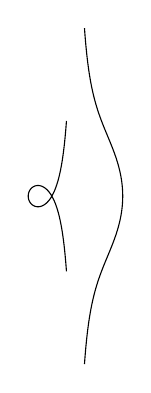
\begin{tikzpicture}
    \def\a{1}
    \def\b{2}
    % {-90+1} so we don't divide by 0. The other +10 are so that we
    % get the picture we want. See the next tikzpicture for a (worse) variant.
    \draw[scale=0.3,domain={-90+11}:{90-11},smooth,variable=\t,samples=180] plot ({\a + \b * cos(\t)}, {\a * tan(\t) + \b * sin(\t)});
    \draw[scale=0.3,domain={-90+11}:{90-11},smooth,variable=\t,samples=180] plot ({\a - \b * cos(\t)}, {\a * tan(\t) - \b * sin(\t)});
  \end{tikzpicture} \hfill
  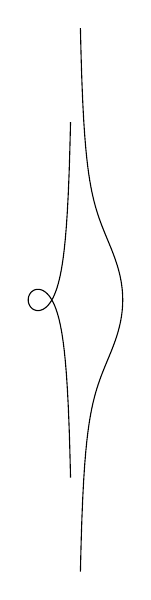
\begin{tikzpicture}
    \def\a{1}
    \def\b{2}
    \draw[scale=0.3,domain={-90+6}:{90-6},smooth,variable=\t,samples=180] plot ({\a + \b * cos(\t)}, {\a * tan(\t) + \b * sin(\t)});
    \draw[scale=0.3,domain={-90+6}:{90-6},smooth,variable=\t,samples=180] plot ({\a - \b * cos(\t)}, {\a * tan(\t) - \b * sin(\t)});
  \end{tikzpicture}
  \caption{Example 2.2: Nicomedes' Conchoid, auto-plot}
\end{figure}
\end{frame}


% -----------------------------------------------------------------
% EXEMPLU 2.3: f(x)=|sin(x)|*exp(-sin(x)), esantionare implicita.
% Aici aratam cum arata un grafic atunci cand nu cerem smooth/samples mare.
% "smooth" NU adauga puncte noi reale; doar uneste mai estetic punctele deja
% evaluate. Daca ai putine samples, curba poate parea frumoasa dar inexacta.
% "samples" controleaza cate puncte sunt evaluate din functie pe domeniu.
% Mai multe samples = fidelitate mai buna, dar compilare mai lenta.
% -----------------------------------------------------------------
\begin{frame}
  \begin{figure}
    \center
    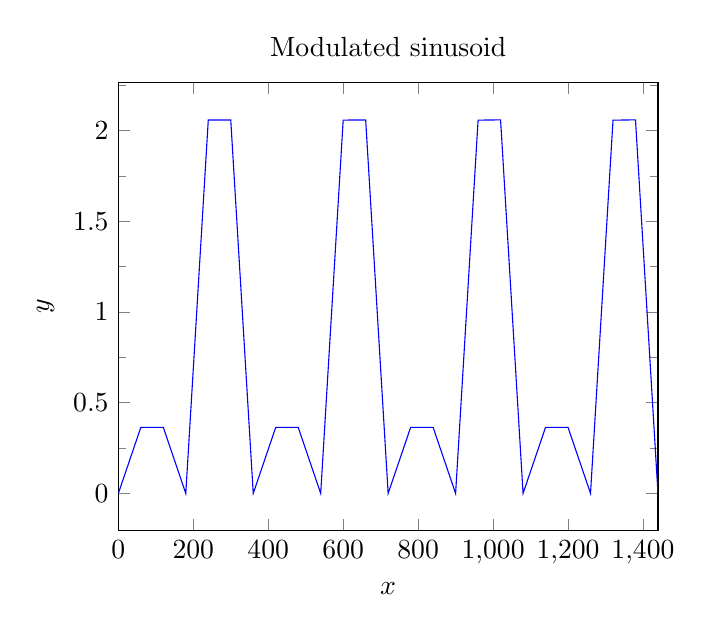
\begin{tikzpicture}
      \begin{axis}[
        title=Modulated sinusoid,
        xlabel={$x$},
        ylabel={$y$},
        domain={0}:{8 * 180}, %8 * pi
        xmin=0, xmax= {8 * 180}, %the actual limits of the plot
        minor y tick num=1, %how many unlabeled ticks between labeled ticks
        ]
        \addplot [blue] {abs(sin(x)) * exp(-sin(x))};
    \end{axis} 
    \end{tikzpicture}
    \caption{Example 2.3: Modulated sinusoid, using PGFPlots. Rough.}
  \end{figure}
\end{frame}

% -----------------------------------------------------------------
% EXEMPLU 2.4: Acelasi grafic, dar cu "smooth".
% Smooth doar interpoleaza vizual; nu creste automat fidelitatea numerica.
% Diferenta practica intre samples uzuale:
%  - samples=100: rapid, bun pentru preview; pot aparea colturi/artefacte.
%  - samples=1000: de obicei echilibru bun calitate/timp.
%  - samples=10000: foarte fin pe functii dificile, dar cost mare la compilare.
% Regula: cresti samples cand vezi rupturi/aliasing, nu "din reflex".
% -----------------------------------------------------------------
\begin{frame}
  \begin{figure}
    \center
    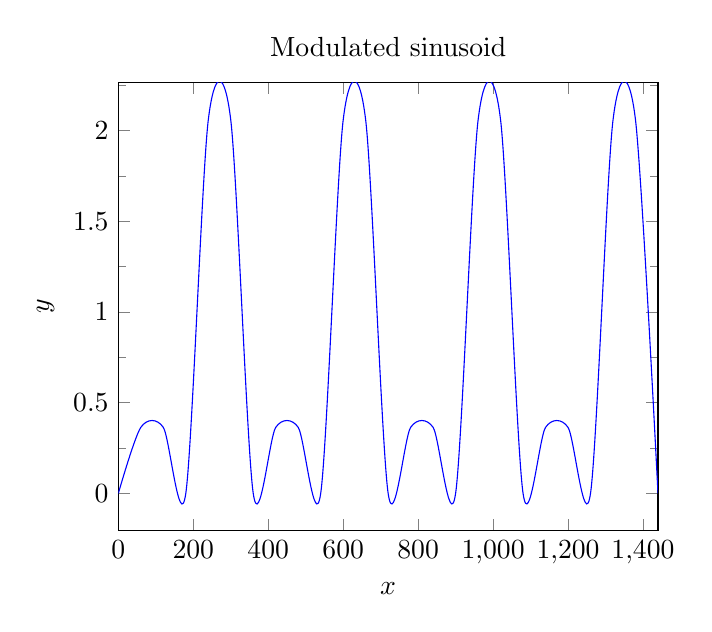
\begin{tikzpicture}
      \begin{axis}[
        title=Modulated sinusoid,
        xlabel={$x$},
        ylabel={$y$},
        domain={0}:{8 * 180}, %8 * pi
        xmin=0, xmax= {8 * 180}, %the actual limits of the plot
        minor y tick num=1, %how many unlabeled ticks between labeled ticks
        smooth,
        ]
        \addplot [blue] {abs(sin(x)) * exp(-sin(x))};
    \end{axis} 
    \end{tikzpicture}
    \caption{Example 2.4: Modulated sinusoid, using PGFPlots. Rough, artificially smoothed.}
  \end{figure}
\end{frame}

% -----------------------------------------------------------------
% EXEMPLU 2.5: Acelasi grafic, "smooth" + samples mare.
% Aceasta este varianta corecta pentru curba mai fina si mai stabila.
% -----------------------------------------------------------------
\begin{frame}
  \begin{figure}
    \center
    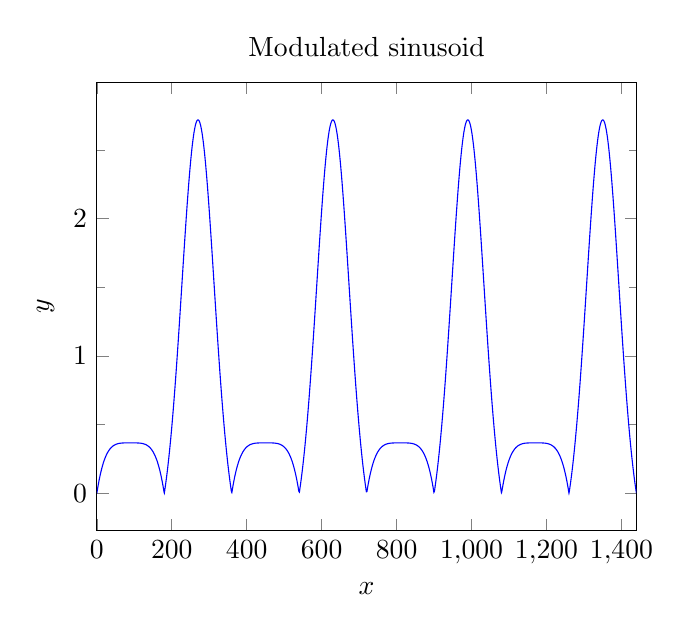
\begin{tikzpicture}
      \begin{axis}[
        title=Modulated sinusoid,
        xlabel={$x$},
        ylabel={$y$},
        domain={0}:{8 * 180}, %8 * pi
        xmin=0, xmax= {8 * 180}, %the actual limits of the plot
        minor y tick num=1, %how many unlabeled ticks between labeled ticks
        smooth,
        samples=1000,
        ]
        \addplot [blue] {abs(sin(x)) * exp(-sin(x))};
    \end{axis} 
    \end{tikzpicture}
    \caption{Example 2.5: Modulated sinusoid, using PGFPlots. Better sampled.}
  \end{figure}
\end{frame}


% -----------------------------------------------------------------
% TASK 2: Circle Concoid (Limaçon / Pascal's Snail), marit pe pagina.
% Formula folosita in cerinta:
%   x = 2*(a*cos(t)+b)*cos(t)
%   y = 2*(a*cos(t)+b)*sin(t)
% CUM:
%   - setam a=0.3, b=0.2
%   - parcurgem t pe [0,360]
%   - scalam sistemul de axe TikZ (x,y) ca sa ocupe mai mult din frame.
% -----------------------------------------------------------------
\begin{frame}
\begin{figure}
  \center
\begin{tikzpicture}[x=4.8cm,y=4.8cm]
  \def\a{0.3}
  \def\b{0.2}
  \draw[black, very thin, domain=0:360, samples=1000, smooth, variable=\t]
    plot ({2*(\a*cos(\t)+\b)*cos(\t)}, {2*(\a*cos(\t)+\b)*sin(\t)});
\end{tikzpicture}
  \caption{Task 2: Circle Concoid}
\end{figure}
\end{frame}



% -----------------------------------------------------------------
% EXEMPLU 3: Polar simplu (spirala in coordonate polare).
% Sintaxa PGFPlots polar: (unghi, raza).
% Diferența dintre \addplot și \addplot+:
%   - \addplot: traseaza curba cu optiunile plotului curent.
%   - \addplot+: ia stilul curent al ciclului (cycle list) + optiunile locale;
%     util cand vrei stiluri coerente intre mai multe curbe fara sa le scrii manual.
% "mark=none": dezactiveaza simbolurile de punct (cerculete/patrate) si lasa
% doar linia. E util la serii dense, ca sa nu incarci vizual graficul.
% -----------------------------------------------------------------
\begin{frame}
\begin{figure}
  \center
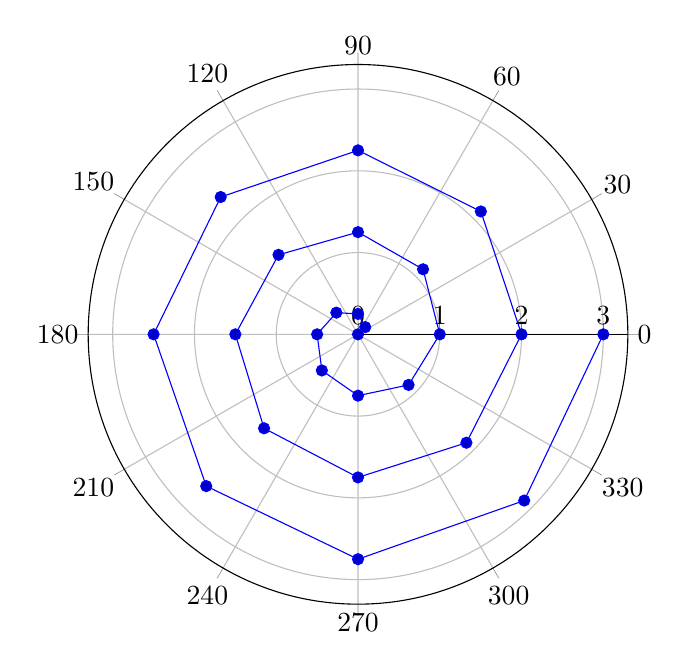
\begin{tikzpicture}
  \begin{polaraxis}
    %try \addplot, notice the difference
    \addplot+ [domain=0:3] (360*x,x); % (angle,radius)
\end{polaraxis} 
\end{tikzpicture}
  \caption{Example 3: Polar plotting}
\end{figure}
\end{frame}


% -----------------------------------------------------------------
% TASK 3: Floare polara ("petale") conform cerintei SG1.
% Formula:
%   r = sin(a*t), cu a=10 (=> 2*a petale pe [0, 2*pi]).
% CUM:
%   - folosim abs(...) pentru petale uniforme (fara alternanta semnului)
%   - domeniu 0..360 grade
%   - samples mare pentru contur continuu/fara intreruperi
% -----------------------------------------------------------------
\begin{frame}
\begin{figure}
  \center
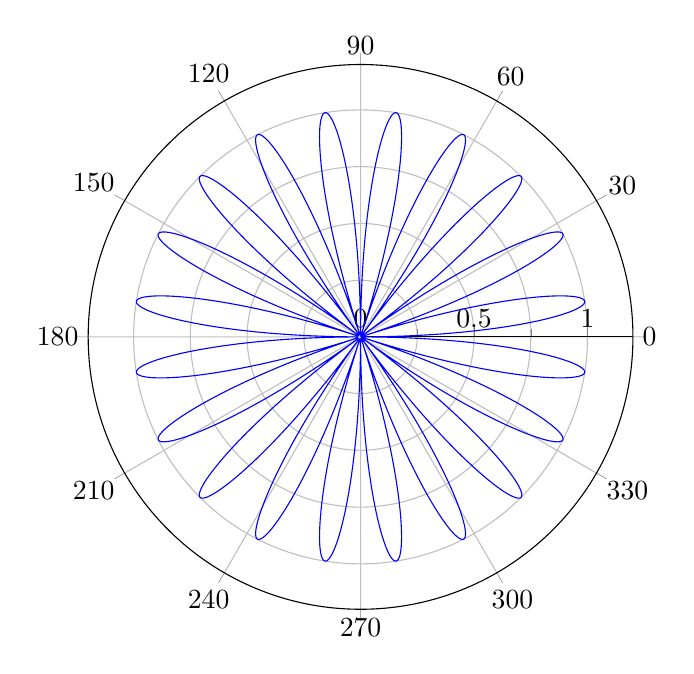
\begin{tikzpicture}
  \begin{polaraxis}[
    ymin=0,
    ymax=1.2,
    xtick={0,30,...,330},
    ytick={0,0.5,1},
    grid=both,
    minor y tick num=1,
    width=8.5cm,
  ]
    \addplot [blue, smooth, domain=0:360, samples=2200] {abs(sin(10*x))};
  \end{polaraxis}
\end{tikzpicture}
  \caption{Task 3: Polar plotting}
\end{figure}
\end{frame}

% -----------------------------------------------------------------
% EXEMPLU 4: Mix date punctuale + date din CSV (mpg.csv).
% -----------------------------------------------------------------
\begin{frame}
  \begin{figure}
    \center
    \begin{tikzpicture}
      \begin{axis} [
        title=Miles per gallon,
        xlabel=hosepower,
        ylabel=mpg,
        ]
        \addplot coordinates {
          (140, 18)
          (140, 17)
          (150, 16)
          (180, 15)
          (220, 14)
        };
        % "only marks" = afiseaza doar puncte.
        % Daca vrei invers (doar linie), folosesti de regula mark=none.
        % Exemplu: \addplot [x=horsepower,y=mpg,col sep=comma,mark=none] {mpg.csv};
        \addplot table [x=horsepower, y=mpg, col sep=comma, only marks] {mpg.csv};
    \end{axis} 
    \end{tikzpicture}
    \caption{Example 4: Plotting datafiles, and coordinates.}
  \end{figure}
\end{frame}

% -----------------------------------------------------------------
% TASK 4 + TASK 5 (vizual): nor de puncte + regresie polinomiala de grad 2.
% CUM:
%   - desenam puncte albastre (simulare de nor de date de tip auto-mpg)
%   - suprapunem curba rosie (polinom de grad 2) ca "fit" extern
%   - pastram caption-ul cerut de laborator (regresie explicata separat la lab)
% -----------------------------------------------------------------
\begin{frame}
  \begin{figure}
    \center
    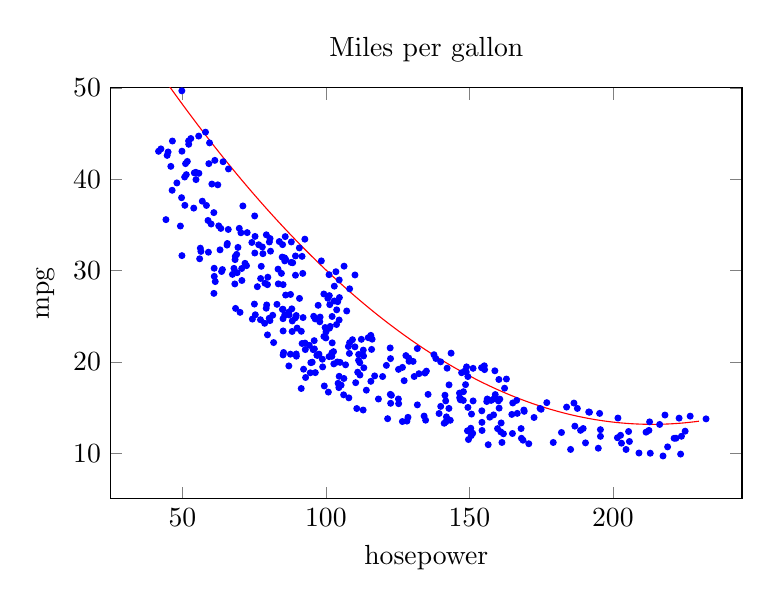
\begin{tikzpicture}
      \begin{axis} [
        title=Miles per gallon,
        xlabel=hosepower,
        ylabel=mpg,
        xmin=25,
        xmax=245,
        ymin=5,
        ymax=50,
        width=9.6cm,
        height=6.8cm,
      ]
        \addplot [blue, only marks, mark=*, mark size=1.05pt, samples=180, domain=45:110]
          ({x + 16*(rnd-0.5)}, {1700/x + 8 + 12*(rnd-0.5)});
        \addplot [blue, only marks, mark=*, mark size=1.05pt, samples=140, domain=80:165]
          ({x + 12*(rnd-0.5)}, {1450/x + 6 + 9*(rnd-0.5)});
        \addplot [blue, only marks, mark=*, mark size=1.05pt, samples=70, domain=140:230]
          ({x + 10*(rnd-0.5)}, {1100/x + 7 + 5*(rnd-0.5)});
        \addplot [red, thin, smooth, samples=300, domain=40:230]
          {0.00130719*x^2 - 0.558823*x + 72.8758};
      \end{axis}
    \end{tikzpicture}
    \caption{4: Plotting datafiles. Make sure to clean data, and regress it externally. Here, a $2^{nd}$ degree polynomial function was fitted in R.}
  \end{figure}
\end{frame}



\end{document}